\documentclass[10pt,a4paper]{article}
\usepackage[T1]{fontenc}
\usepackage[utf8]{inputenc}
\usepackage[french]{babel}
\usepackage{lmodern,microtype}
\usepackage[a4paper,margin=2cm,headheight=15pt]{geometry}
\usepackage{amsmath,amssymb}
\usepackage{graphicx,booktabs,tabularx,float,caption}
\usepackage[table]{xcolor}
\usepackage{enumitem,fancyhdr,tikz,tcolorbox,titlesec,listings}
\usepackage{hyperref}
\definecolor{Encre}{HTML}{243447}
\definecolor{Bleu}{HTML}{357AB3}
\definecolor{Pale}{HTML}{F0F7FC}
\definecolor{Gris}{HTML}{627486}
\definecolor{Vert}{HTML}{68AFA5}
\definecolor{Bordeaux}{HTML}{8B1538}
\definecolor{RosePale}{HTML}{FCF6F8}
\hypersetup{colorlinks=true,linkcolor=Bleu,urlcolor=Bleu,citecolor=Bleu,
 pdftitle={Clustering sous contrainte d'ordre},
 pdfauthor={Manel LAKROUZ et Sirine BOUGHANEM},bookmarksnumbered=true}
\urlstyle{same}
\graphicspath{{figures/}}
\captionsetup{font=small,labelfont={color=Bleu},skip=6pt}
\renewcommand{\figurename}{Figure}
\renewcommand{\tablename}{Tableau}
\setlength{\parindent}{0pt}
\setlength{\parskip}{4pt}
\setlength{\emergencystretch}{2em}
\setlength{\intextsep}{11pt plus 2pt minus 2pt}
\setlist{leftmargin=1.4em,itemsep=2pt,topsep=4pt}
\renewcommand{\arraystretch}{1.15}
\setcounter{tocdepth}{2}
\addto\captionsfrench{\renewcommand{\contentsname}{Sommaire}\renewcommand{\tablename}{Tableau}}
\titleformat{\section}{\large\sffamily\bfseries\color{Encre}}
 {\color{Bleu}\thesection}{0.65em}{}[\vspace{2pt}{\color{Bleu!25}\titlerule}]
\titleformat{\subsubsection}{\normalsize\sffamily\bfseries\color{Bleu}}{}{0pt}{}
\titlespacing*{\subsubsection}{0pt}{10pt}{4pt}
\titleformat{\subsection}{\normalsize\sffamily\bfseries\color{Encre}}
 {\color{Bleu}\thesubsection}{0.65em}{}
\titlespacing*{\section}{0pt}{12pt}{7pt}
\titlespacing*{\subsection}{0pt}{9pt}{4pt}
\newtcolorbox{boitebilan}{colback=Pale,colframe=Bleu!45,boxrule=0pt,leftrule=2pt,
 arc=1.5mm,left=9pt,right=9pt,top=7pt,bottom=7pt,before skip=7pt,after skip=7pt}
\newcommand{\synthese}[1]{\begin{boitebilan}\small #1\end{boitebilan}}
\pagestyle{fancy}
\fancyhf{}
\fancyhead[L]{\small\sffamily\color{Gris}Clustering sous contrainte d'ordre}
\fancyhead[R]{\small\sffamily\color{Gris}Université Paris Cité}
\fancyfoot[L]{\footnotesize\sffamily\color{Gris}M. Lakrouz \quad / \quad S. Boughanem}
\fancyfoot[R]{\small\sffamily\color{Bleu}\thepage}
\renewcommand{\headrulewidth}{0.3pt}
\lstset{language=Python,basicstyle=\ttfamily\small,keywordstyle=\color{Bleu},
 commentstyle=\color{Gris},backgroundcolor=\color{Pale},frame=single,
 rulecolor=\color{Bleu!25},framerule=0.4pt,xleftmargin=6pt,xrightmargin=6pt,
 framexleftmargin=5pt,framexrightmargin=5pt,aboveskip=9pt,belowskip=9pt,
 showstringspaces=false,columns=fullflexible,keepspaces=true,breaklines=true}
\begin{document}
\hypersetup{pageanchor=false}
\begin{titlepage}
\begin{tikzpicture}[remember picture,overlay]
 \fill[RosePale] (current page.south west) rectangle ([yshift=5.7cm]current page.south east);
 \fill[Bordeaux!65] (current page.north west) rectangle ([xshift=0.12cm]current page.south west);
\end{tikzpicture}
\sffamily\vspace*{0.15cm}
% Logo officiel : https://u-paris.fr/wp-content/uploads/2022/03/UniversiteParisCite_logo_horizontal_couleur_RVB.pdf
\begin{minipage}[c]{0.60\textwidth}
 
\includegraphics[width=6.5cm]{assets/universite-paris-cite-logo.pdf}
\end{minipage}\hfill
\begin{minipage}[c]{0.35\textwidth}
 \raggedleft
 {\normalsize\bfseries\color{Encre}Master 2 MLSD}\par
 \vspace{0.15cm}
 {\small\color{Gris}Année universitaire}\par
 {\small\color{Gris}2026--2027}
\end{minipage}
\vspace{0.6cm}
{\color{Bordeaux!25}\rule{\linewidth}{0.6pt}}\par
\vspace{2.1cm}
\begingroup
\centering
{\small\bfseries\color{Bordeaux}RAPPORT DE PROJET}\par
\vspace{0.7cm}
{\fontsize{34}{40}\selectfont\bfseries\color{Encre}
Clustering sous\par contrainte d'ordre}\par
\vspace{0.75cm}
{\fontsize{17}{23}\selectfont\color{Gris}Programmation dynamique de Fisher}\par
\vspace{0.3cm}
{\normalsize\color{Gris}Comparaison avec K-means et la CAH de Ward}\par
\vspace{1.05cm}
\begin{tikzpicture}
 \fill[Bordeaux!20,rounded corners=1.5pt] (0,0) rectangle (2.1,0.12);
 \fill[Bordeaux!50,rounded corners=1.5pt] (2.25,0) rectangle (4.35,0.12);
 \fill[Bleu!35,rounded corners=1.5pt] (4.5,0) rectangle (6.6,0.12);
 \fill[Bleu!65,rounded corners=1.5pt] (6.75,0) rectangle (8.85,0.12);
\end{tikzpicture}\par
\vfill
{\small\bfseries\color{Bordeaux}RÉALISÉ PAR}\par
\vspace{0.4cm}
\begin{tcolorbox}[width=0.86\textwidth,colback=white,colframe=Bordeaux!20,
 boxrule=0.5pt,arc=2mm,left=12pt,right=12pt,top=13pt,bottom=13pt]
\centering
\begin{minipage}[t]{0.47\linewidth}
 \centering
 {\normalsize\color{Gris}Manel}\par\smallskip
 {\large\bfseries\color{Encre}LAKROUZ}
\end{minipage}\hfill
\begin{minipage}[t]{0.47\linewidth}
 \centering
 {\normalsize\color{Gris}Sirine}\par\smallskip
 {\large\bfseries\color{Encre}BOUGHANEM}
\end{minipage}
\end{tcolorbox}
\par\endgroup
\vspace{0.7cm}

{\color{Bordeaux!20}\rule{\linewidth}{0.4pt}}\par
\vspace{0.25cm}
{\small\color{Gris}Université Paris Cité\hfill Novembre 2026}\par
\vspace*{0.4cm}
\end{titlepage}
\pagenumbering{roman}
\hypersetup{pageanchor=true}
\begingroup\small\tableofcontents\endgroup
\clearpage
\phantomsection
\addcontentsline{toc}{section}{Résumé}
\vspace*{1.4cm}
\begin{center}
\begin{minipage}{0.90\textwidth}
\section*{Résumé}
\fontsize{11.5}{17}\selectfont
\vspace{0.5cm}
Ce projet étudie la classification sous contrainte d'ordre, qui consiste à
découper une séquence en segments contigus et homogènes. Nous implémentons
l'algorithme de Fisher par programmation dynamique, puis le validons à l'aide
de 40 tests unitaires, dont une comparaison à une recherche exhaustive sur de
petites séquences. Ses résultats sont comparés à ceux de K-means et de la CAH de
Ward à l'aide de l'inertie, de l'indice de Rand ajusté et de la silhouette.
\par\smallskip
Sur les 160 observations simulées de \texttt{sequencesimu}, la méthode du coude
conduit à quatre segments, dont deux présentent des profils moyens proches.
Sur les 140 observations du fichier \texttt{aiguillage}, décrites par 552 variables,
Fisher retrouve exactement les quatre classes de référence ; K-means et Ward
présentent respectivement trois et huit désaccords. Ces expériences montrent
l'intérêt de l'ordre pour segmenter une séquence et distinguent compacité
géométrique et accord avec une partition connue.
\par\medskip
L'expérience complémentaire de mélange des lignes souligne que le résultat de
Fisher dépend de la pertinence de l'ordre initial. La méthode vise ainsi la
segmentation de périodes successives, tandis que les méthodes non contraintes
décrivent les ressemblances entre observations, quelle que soit leur position.
\par\bigskip
\begin{boitebilan}
\textbf{Mots-clés :} classification sous contrainte d'ordre ; segmentation ;
programmation dynamique ; Fisher ; K-means ; CAH de Ward.
\end{boitebilan}
\end{minipage}
\end{center}
\clearpage
\pagenumbering{arabic}
\fontsize{10.5}{12.7}\selectfont
\section{Introduction}
La classification non supervisée regroupe des observations $x_1,\ldots,x_n\in
\mathbb{R}^p$ en classes homogènes. K-means et la CAH peuvent réunir des
observations éloignées dans une séquence : leur position n'est pas une contrainte.
Pour des mesures ordonnées dans le temps ou dans l'espace, on cherche au contraire
à identifier des \textbf{segments successifs}, délimités par $K-1$ ruptures.

L'algorithme de Fisher\cite{fisher} résout ce problème exactement par
programmation dynamique. Nous présentons son implémentation et sa validation,
puis comparons ses partitions à celles de K-means et de Ward. Le rapport suit les
questions du sujet : choix de $K$ sur les données simulées, puis segmentation
des données réelles avec $K=4$ et comparaison aux classes connues.

\section{L'algorithme de Fisher}

\subsection{Formulation du problème}

Pour un segment $(x_a,\dots,x_b)$ avec $a\le b$, on définit son
\textbf{diamètre} comme son inertie :
\[
D(a,b) = \sum_{i=a}^{b} \lVert x_i - \mu_{ab} \rVert^2,
\qquad \mu_{ab} = \frac{1}{b-a+1}\sum_{i=a}^{b} x_i .
\]
Une partition en $K$ segments est entièrement déterminée par les débuts des
segments $2,\dots,K$, notés $1 < t_1 < t_2 < \dots < t_{K-1} \le n$. Le critère
à minimiser est l'inertie intra-classe :
\[
C = \sum_{k=1}^{K} D(t_{k-1}, t_k-1), \qquad t_0=1,\quad t_K=n+1.
\]
Le nombre de partitions possibles est $\binom{n-1}{K-1}$, ce qui interdit une
énumération exhaustive dès que $n$ est grand (pour $n=160$ et $K=4$, $657\,359$
partitions ; pour $K=10$, plus de $10^{13}$).

\subsection{Programmation dynamique}

L'algorithme repose sur le principe de Bellman : \emph{toute sous-partition
d'une partition optimale est optimale}. Notons $M(i,k)$ le critère optimal pour
découper les $i$ premières observations en $k$ segments. On a alors
\[
M(i,1) = D(1,i), \qquad
M(i,k) = \min_{k \le t \le i} \bigl[ M(t-1, k-1) + D(t, i) \bigr], \quad 2\le k \le K,\ k\le i \le n,
\]
où $t$ est le début du dernier segment. L'algorithme comporte quatre étapes :
\begin{enumerate}
  \item \textbf{Calcul de la matrice triangulaire supérieure} $D(a,b)$ pour $1\le a\le b\le n$.
  \item \textbf{Calcul récursif des critères optimaux} $M(i,k)$, en conservant
        dans une matrice $A(i,k)$ l'indice $t$ qui réalise le minimum.
  \item \textbf{Remontée (\emph{backtracking})} : $t_{K-1} = A(n,K)$, puis
        $t_{k-1} = A(t_k - 1, k)$ pour $k = K-1,\dots,2$.
  \item \textbf{Construction des labels} : les observations de $t_{k-1}$ à $t_k - 1$
        reçoivent le label $k$ (avec $t_0=1$ et $t_K = n+1$).
\end{enumerate}
Le critère optimal est $C = M(n,K)$. L'étape 2 coûte $O(Kn^2)$ opérations ;
le calcul de $D$ coûte $O(n^3p)$ dans notre implémentation directe. Des sommes
cumulées permettraient de le ramener à $O(n^2p)$.

\subsection{Propriétés}

\begin{itemize}
  \item \textbf{Optimalité globale} : contrairement à K-means, dont le résultat
        dépend de l'initialisation et ne garantit pas l'optimum global, Fisher fournit la meilleure
        partition en $K$ segments contigus.
  \item \textbf{Déterminisme} : à données, ordre et $K$ fixés, le résultat est
        toujours le même.
  \item \textbf{Solutions pour tout $k\le K$} : la matrice $M$ contient $M(n,k)$
        pour tous les $k\le K$, ce qui facilite le choix du nombre de segments.
  \item \textbf{Dépendance à l'ordre} : la méthode n'a de sens que si l'ordre des
        observations porte une information.
\end{itemize}

% =====================================================================
\clearpage
\begingroup
\fontsize{11}{14}\selectfont
\section{Implémentation et validation}

\subsection{Organisation du code}

L'ensemble des fonctions est regroupé dans le module \texttt{utils.py}. Les
observations sont les lignes de la matrice $X$ ; les indices de segments suivent
la convention mathématique (à partir de 1) et les labels renvoyés vont de $1$ à $K$.

\begin{table}[H]
\centering
\small
\begin{tabular}{@{}lll@{}}
\toprule
\textbf{Fonction} & \textbf{Rôle} & \textbf{Sortie} \\
\midrule
\texttt{diam(X, a, b)} & diamètre $D(a,b)$ du segment $(x_a,\dots,x_b)$ & réel \\
\texttt{clustfisher(X, K)} & segmentation optimale de Fisher & ruptures, labels, $C$ \\
\texttt{clustkmeans(X, K)} & K-means, 10 initialisations, graine fixe & labels, inertie \\
\texttt{clustward(X, K)} & CAH avec le critère de Ward & labels, inertie \\
\texttt{inertie(X, cluster)} & inertie intra-classe d'une partition & réel \\
\texttt{compare\_partitions(c1, c2)} & indice de Rand ajusté (ARI) & réel \\
\texttt{silhouette(X, cluster)} & silhouette moyenne (distance euclidienne) & réel \\
\bottomrule
\end{tabular}
\caption{Fonctions du module \texttt{utils.py}.}
\end{table}

Le cœur de \texttt{clustfisher} est vectorisé sur les débuts possibles $t$ du
dernier segment. La matrice $A$ conserve le meilleur choix pour reconstruire
ensuite les ruptures. L'extrait suivant reprend ces deux étapes :

\begin{lstlisting}
for k in range(2, K + 1):
    for i in range(k, n + 1):
        ts = np.arange(k, i + 1)  # debuts possibles
        valeurs = M[ts - 1, k - 1] + D[ts, i]
        M[i, k] = valeurs.min()
        A[i, k] = ts[np.argmin(valeurs)]

k = K - 1
m = n
while k >= 1:
    t[k] = A[m, k + 1]
    m = t[k] - 1
    k -= 1
\end{lstlisting}

Le tableau \texttt{ts} évite une troisième boucle Python explicite. La remontée
part du dernier segment et retrouve les frontières en sens inverse ; les labels
sont ensuite construits à partir de ces bornes.

K-means et Ward sont appelés depuis \texttt{scikit-learn}. Pour comparer
équitablement les trois méthodes, l'inertie de K-means et de Ward est recalculée
avec la fonction \texttt{inertie}, qui utilise exactement le même critère que Fisher.

\subsubsection*{K-means}
K-means alterne affectation au centre le plus proche et mise à jour des moyennes
des groupes. Dix initialisations sont testées et la solution de plus faible
inertie est retenue, avec une graine fixée à 0.

\subsubsection*{CAH de Ward}
Ward fusionne successivement les groupes en limitant l'augmentation de l'inertie,
puis la hiérarchie est coupée à $K$ classes. Comme K-means, elle n'impose pas
la contiguïté des groupes dans la séquence.


\clearpage
\subsection{Critères de comparaison}

\begin{itemize}
  \item \textbf{Inertie intra-classe} $\sum_k \sum_{i\in C_k}\lVert x_i-\mu_k\rVert^2$ :
        mesure la compacité des classes (plus faible = plus compact).
  \item \textbf{Indice de Rand ajusté (ARI)} : mesure l'accord entre deux partitions,
        indépendamment de la numérotation des classes. Il vaut 1 pour deux
        partitions identiques et autour de 0 au niveau attendu au hasard ; il peut être négatif.
  \item \textbf{Silhouette moyenne} : pour chaque point,
        $s_i = (b_i - a_i)/\max(a_i,b_i)$, où $a_i$ est la distance moyenne aux
        autres points de sa classe et $b_i$ la distance moyenne à la classe voisine la plus
        proche. Une valeur proche de 1 indique des classes bien séparées.
  \item \textbf{Nombre de changements de classe} le long de la séquence : il vaut
        exactement $K-1$ pour une segmentation en blocs contigus.
\end{itemize}

Ces critères répondent à des questions distinctes. L'inertie et la silhouette
décrivent la géométrie des groupes ; l'ARI compare des appartenances ; le nombre
de changements décrit leur organisation dans la séquence. Une silhouette élevée
ne suffit donc pas à conclure qu'une méthode retrouve les périodes recherchées.
Les inerties sont comparées à données et nombre de classes identiques.

\subsection{Protocole expérimental}
Pour chaque fichier, nous conservons l'ordre initial des lignes et utilisons les
mêmes variables brutes pour les trois méthodes. Le protocole suit quatre étapes :
\begin{enumerate}
 \item charger les variables explicatives et vérifier les dimensions ;
 \item choisir $K$ par la méthode du coude sur \texttt{sequencesimu}, ou fixer
       $K=4$ conformément au sujet sur \texttt{aiguillage} ;
 \item calculer les partitions de Fisher, K-means et Ward, puis leurs critères ;
 \item confronter les scores aux représentations dans la séquence et dans le plan.
\end{enumerate}
Sur \texttt{aiguillage}, la dernière colonne est isolée avant toute classification.
Elle sert à l'évaluation et à la description des classes de référence. Lorsque
les groupes sont renumérotés pour lire les désaccords, seule leur étiquette change,
pas l'affectation des observations. Sur \texttt{sequencesimu}, en l'absence de
vérité fournie, l'ARI avec Fisher mesure un accord entre méthodes et non une
exactitude de classification.

\subsection{Tests unitaires}

Deux fichiers de tests (\texttt{unittest}) vérifient le module, soit
\textbf{40 tests, tous réussis}.
\begin{itemize}
  \item \texttt{testutils.py} (22 tests) : valeurs connues de \texttt{diam} en
        dimension 1 et $p$, égalité $D(a,b) = (b-a+1)\times$ variance, cas $K=1$ et
        $K=n$ (critère nul), paliers évidents, cohérence entre ruptures et labels,
        égalité entre $C$ et la somme des diamètres, décroissance de $C$ en $K$,
        rejet de certaines valeurs invalides de $K$, et surtout \textbf{comparaison avec une
        recherche exhaustive} sur de petites séquences, qui vérifie
        l'optimalité sur ces cas de petite taille.
  \item \texttt{testcomparaison.py} (18 tests) : K-means et Ward sur des groupes
        séparés ou non contigus, reproductibilité de K-means, invariance de l'ARI
        aux permutations de labels, inertie de Fisher, valeur connue de la silhouette.
\end{itemize}

% =====================================================================
\clearpage
\endgroup
\section[Données simulées : sequencesimu]{Données simulées : \texttt{sequencesimu} (question 2)}

\subsection{Données}

La séquence comporte $n=160$ observations en dimension $p=2$ (\texttt{var1},
\texttt{var2}). Cette fois, \textbf{le nombre de segments est inconnu} et
\textbf{aucune partition de référence n'est fournie}.

\begin{figure}[H]
\centering
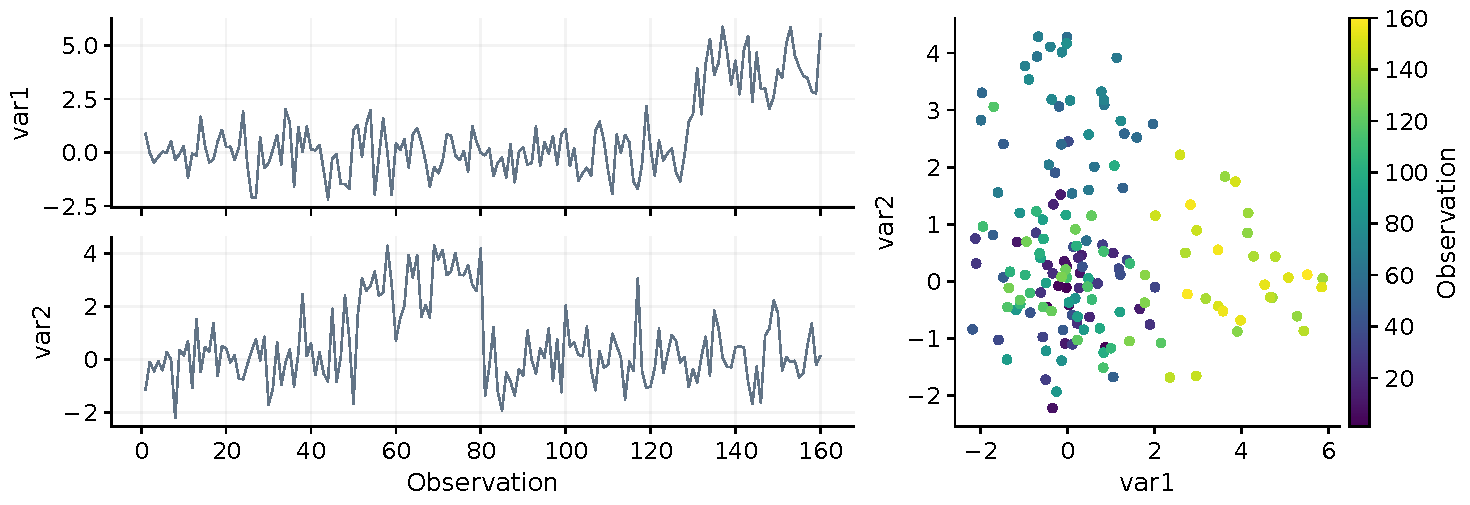
\includegraphics[width=\linewidth,height=4.8cm,keepaspectratio]{seq_donnees}
\caption{Les deux variables dans l'ordre de la séquence (à gauche) et nuage de
points coloré selon la position (à droite).}
\label{fig:seq-donnees}
\end{figure}

On distingue des changements de niveau : \texttt{var2} monte vers 3 entre les
observations 50 et 80, \texttt{var1} monte vers 4 en fin de séquence. Le nuage
montre trois zones, autour de $(0,0)$, $(0,3)$ et $(4,0)$, la zone $(0,0)$ étant
visitée au début \emph{et} au milieu de la séquence.

\subsection{Choix du nombre de segments par la méthode du coude}

Nous calculons le critère optimal $C(K)$ de Fisher pour $K=1,\dots,15$.
$C(K)$ décroît nécessairement avec $K$ ; on cherche donc la valeur au-delà de
laquelle un segment supplémentaire ne réduit plus que faiblement le critère.

\begin{table}[H]
\centering
\small
\begin{tabular}{@{}crrrl@{}}
\toprule
$K$ & $C(K)$ & Gain $C(K-1)-C(K)$ & Gain relatif & Ruptures \\
\midrule
1 & 884,1 & -- & -- & -- \\
2 & 503,6 & 380,6 & 43,0\,\% & 131 \\
3 & 462,0 & 41,6 & 8,3\,\% & 81, 131 \\
\textbf{4} & \textbf{300,6} & \textbf{161,4} & \textbf{34,9\,\%} & \textbf{51, 81, 131} \\
5 & 292,4 & 8,2 & 2,7\,\% & 51, 81, 129, 133 \\
6 & 285,5 & 6,9 & 2,4\,\% & 51, 69, 81, 129, 133 \\
\bottomrule
\end{tabular}
\caption{Critère de Fisher et gains pour les premières valeurs de $K$.}
\label{tab:coude}
\end{table}

\begin{figure}[H]
\centering
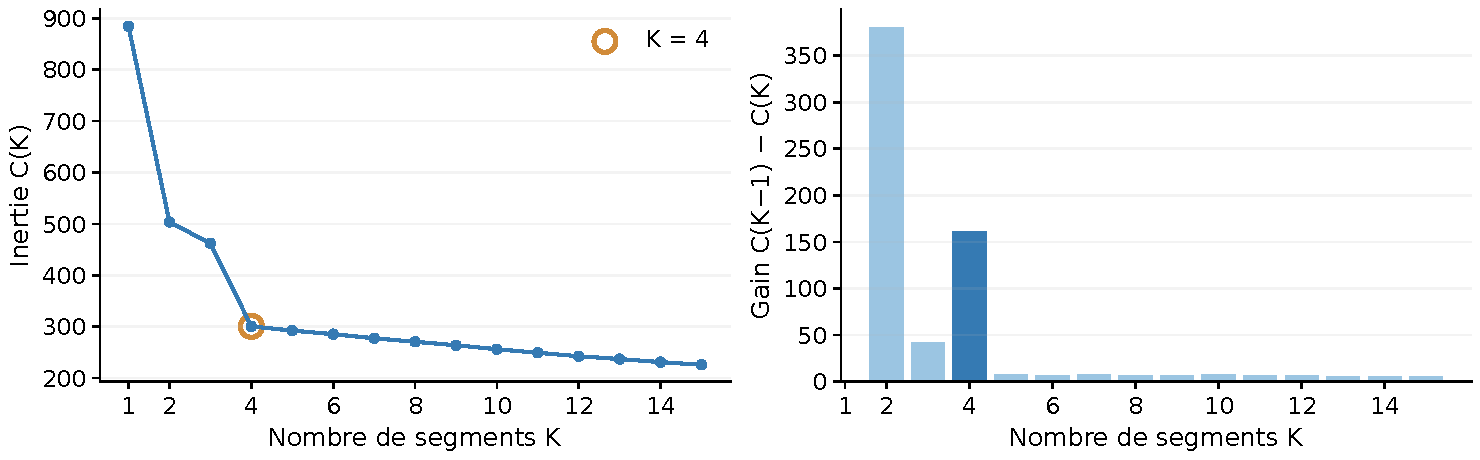
\includegraphics[width=\linewidth,height=4.7cm,keepaspectratio]{seq_coude}
\caption{Méthode du coude : critère $C(K)$ (à gauche) et gain apporté par le
$K$-ième segment (à droite).}
\label{fig:coude}
\end{figure}

Après $K=4$, les gains se limitent à environ 5 à 8 unités sur la plage étudiée,
contre 161,4 entre 3 et 4. La rupture en 51 sépare les deux niveaux de
\texttt{var2} encore réunis dans le segment 1--80 pour $K=3$.
Les gains ultérieurs suggèrent surtout l'ajustement de variations résiduelles.
\textbf{Nous retenons $K=4$.}

\clearpage
\subsection{Segmentation de Fisher}

\begin{table}[H]
\centering
\small
\begin{tabular}{@{}ccrrrrr@{}}
\toprule
Segment & Observations & Effectif & Moy. var1 & Moy. var2 & É.-t. var1 & É.-t. var2 \\
\midrule
1 & 1--50    & 50 & $-0{,}06$ & $0{,}00$ & 0,98 & 0,95 \\
2 & 51--80   & 30 & $0{,}09$ & $2{,}93$ & 0,98 & 0,93 \\
3 & 81--130  & 50 & $-0{,}10$ & $-0{,}06$ & 0,93 & 0,95 \\
4 & 131--160 & 30 & $3{,}88$ & $0{,}16$ & 1,12 & 0,94 \\
\bottomrule
\end{tabular}
\caption{Description des quatre segments de Fisher ($C(4) = 300{,}6$).}
\label{tab:segments}
\end{table}

\begin{figure}[H]
\centering
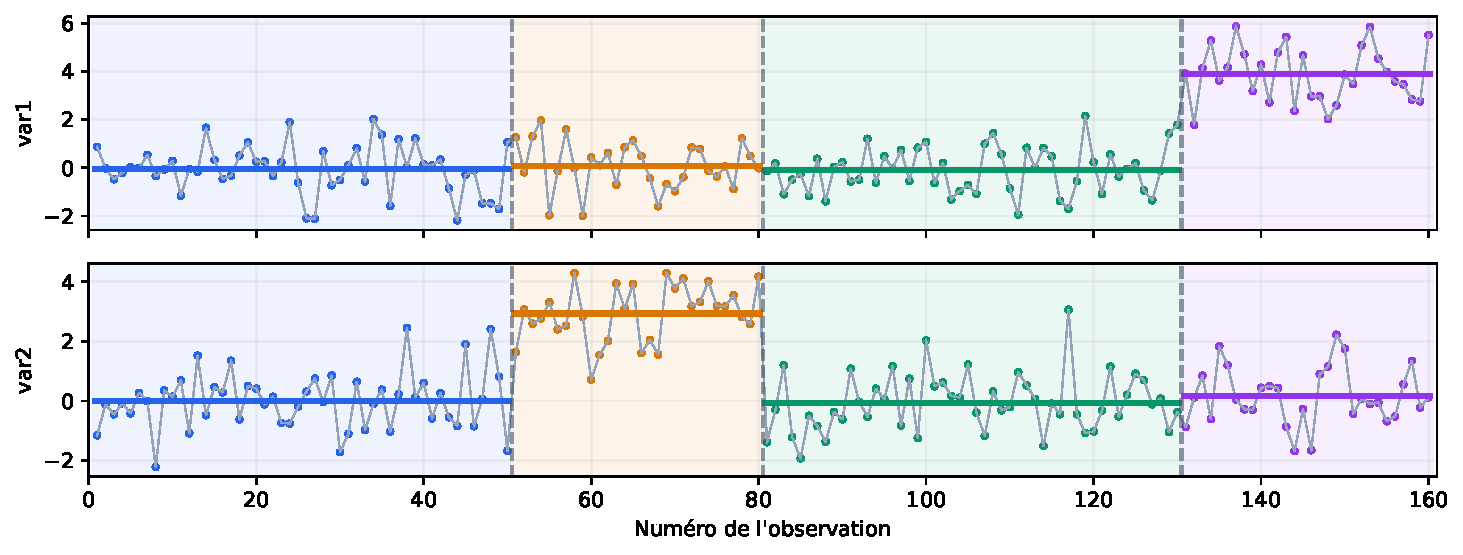
\includegraphics[width=\linewidth,height=8.2cm,keepaspectratio]{seq_fisher}
\caption{Segmentation de Fisher ($K=4$). Les traits pleins indiquent la moyenne
de chaque segment.}
\label{fig:seq-fisher}
\end{figure}

Chaque segment correspond à un régime moyen : $(0,0)$, $(0,3)$, $(0,0)$ et
$(4,0)$. Les écarts-types sont tous proches de 1 : les dispersions sont
comparables et les différences concernent principalement les moyennes. Ces résumés
ne permettent pas d'établir l'égalité des distributions.
Point important, \textbf{les segments 1 et 3 ont des moyennes proches} : Fisher les
distingue uniquement parce qu'ils sont séparés dans le temps par le segment 2.

\subsection{Comparaison avec K-means et la CAH de Ward}

Nous appliquons K-means et Ward avec le même nombre de classes, $K=4$.

\begin{table}[H]
\centering
\small
\begin{tabular}{@{}lrrrr@{}}
\toprule
\textbf{Méthode} & \textbf{Inertie} & \textbf{Silhouette} & \textbf{Changements} & \textbf{ARI avec Fisher} \\
\midrule
Fisher  & 300,6 & 0,155 & 3  & 1,000 \\
K-means & \textbf{202,9} & 0,372 & 75 & 0,390 \\
Ward    & 246,6 & \textbf{0,374} & 45 & 0,392 \\
\bottomrule
\end{tabular}
\caption{Comparaison des trois partitions sur \texttt{sequencesimu} ($K=4$).
L'ARI entre K-means et Ward vaut 0,432.}
\label{tab:seq}
\end{table}

\clearpage
\subsection{Lecture des partitions dans le plan et dans la séquence}
\begin{figure}[H]
\centering
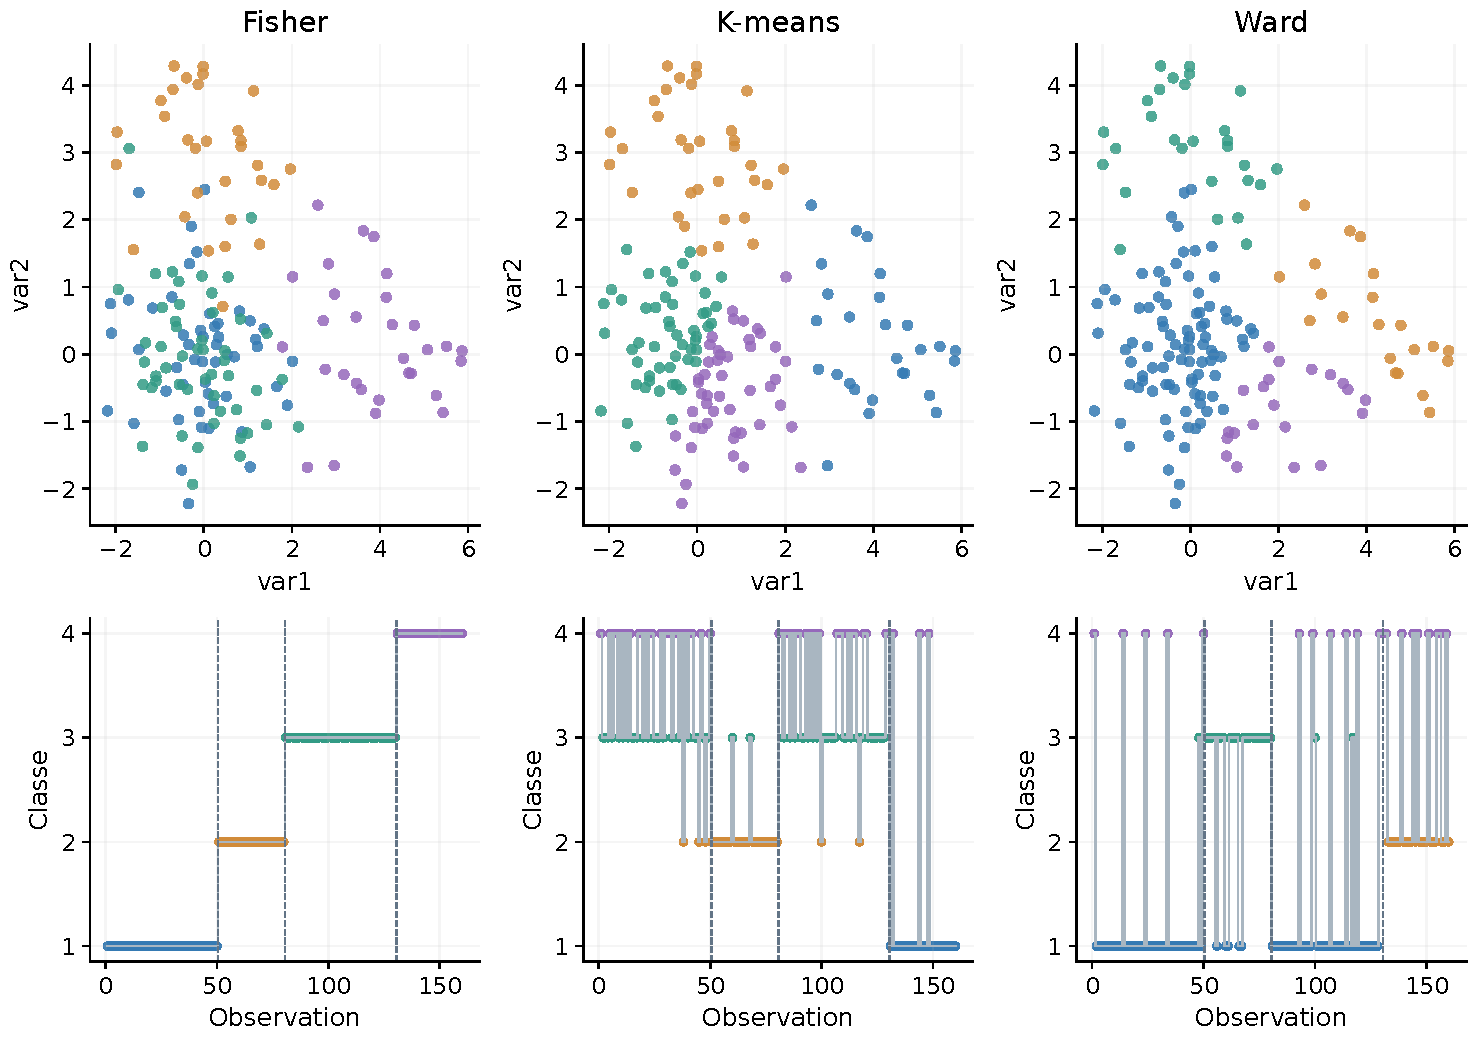
\includegraphics[width=\linewidth,height=12.1cm,keepaspectratio]{seq_partitions}
\caption{Les trois partitions dans le plan (en haut) et le long de la séquence
(en bas). Pointillés : ruptures de Fisher.}
\label{fig:seq-parts}
\end{figure}



\textbf{Lecture des partitions.} Les segments 1 et 3 de Fisher se superposent
dans le plan, alors qu'ils occupent deux périodes distinctes. K-means et Ward
forment des groupes plus compacts mais non contigus : une même couleur peut
apparaître à plusieurs endroits de la séquence. La lecture conjointe des deux
représentations distingue ainsi ressemblance géométrique et succession des périodes.

La ligne inférieure de la figure~\ref{fig:seq-parts} aide à comprendre ces
résultats. Fisher ne change de label qu'aux observations 51, 81 et 131. Le
retour vers la zone proche de $(0,0)$, à partir de l'observation 81, reçoit un
nouveau label parce qu'il commence une nouvelle période, même si son profil
moyen ressemble à celui du premier segment. Il s'agit donc d'une information
sur la position dans la séquence, qui ne se lit pas dans le seul nuage de points.

À l'inverse, K-means et Ward regroupent les observations selon leurs valeurs.
Leurs changements de label correspondent à 76 et 46 plages successives, soit
bien plus que les quatre segments demandés à Fisher. Une meilleure compacité
n'implique donc pas ici une segmentation plus lisible. Les couleurs doivent être
lues au sein de chaque partition : les numéros des groupes ne sont pas directement
comparables d'une méthode à l'autre.

Enfin, aucune classe de référence n'étant fournie pour cette séquence, les
frontières de Fisher restent un résultat de segmentation, et non des ruptures
connues avec lesquelles mesurer une erreur. Le choix de quatre segments repose
sur le coude et sur la cohérence des changements de niveau observés.

\clearpage
\subsection{Comparaison détaillée des appartenances}
Les tableaux croisés précisent comment les observations des segments de Fisher
se répartissent entre les groupes des deux méthodes non contraintes. Les numéros
de groupes sont propres à chaque méthode et n'ont pas d'ordre naturel.

\begin{table}[H]
\centering
\small
\begin{tabular}{@{}c|cccc@{\hspace{1.5cm}}c|cccc@{}}
\multicolumn{5}{c}{\textbf{Fisher $\times$ K-means}} & \multicolumn{5}{c}{\textbf{Fisher $\times$ Ward}} \\
\toprule
Seg. & G1 & G2 & G3 & G4 & Seg. & G1 & G2 & G3 & G4 \\
\midrule
1 & 0 & 3 & 23 & 24 & 1 & 44 & 0 & 1 & 5 \\
2 & 0 & 28 & 2 & 0 & 2 & 5 & 0 & 25 & 0 \\
3 & 0 & 2 & 27 & 21 & 3 & 41 & 0 & 2 & 7 \\
4 & 27 & 0 & 0 & 3 & 4 & 0 & 21 & 0 & 9 \\
\bottomrule
\end{tabular}
\caption{Tableaux croisés entre les segments de Fisher (lignes) et les groupes de
K-means et de Ward (colonnes).}
\label{tab:croises}
\end{table}


\begin{itemize}
  \item \textbf{Compacité.} K-means et Ward ont ici une inertie plus faible et une
        silhouette plus élevée. La superposition des segments 1 et 3 dans le plan
        contribue à la silhouette faible de Fisher (0,155).
  \item \textbf{Structure dans la séquence.} Les 75 et 45 changements de classe
        de K-means et Ward, contre 3 pour Fisher, montrent que leurs groupes
        ne correspondent pas à quatre périodes successives.
  \item \textbf{Appartenances.} K-means retrouve 28 des 30 observations du segment 2
        dans un groupe et 27 des 30 du segment 4 dans un autre. Les segments 1 et 3
        sont mélangés entre plusieurs groupes ; Ward en réunit 85 sur 100 dans G1
        et place notamment des points intermédiaires dans G4.
  \item \textbf{Accord entre méthodes.} L'ARI de 0,432 entre K-means et Ward
        indique des partitions différentes. Avec $K=4$, leurs critères conduisent
        à subdiviser différemment les trois zones géométriques observées.
\end{itemize}

\subsection{Analyse complémentaire : trois régimes, quatre périodes}

Puisque les segments 1 et 3 ont des moyennes proches, nous les avons fusionnés pour
obtenir trois \emph{régimes} et comparé cette partition à K-means et Ward appliqués
avec $K=3$.

\begin{table}[H]
\centering
\small
\begin{tabular}{@{}lc@{}}
\toprule
\textbf{Partition} & \textbf{ARI avec les 3 régimes de Fisher} \\
\midrule
K-means ($K=3$) & \textbf{0,805} \\
Ward ($K=3$)    & 0,634 \\
K-means ($K=4$) & 0,470 \\
Ward ($K=4$)    & 0,641 \\
\bottomrule
\end{tabular}
\caption{Accord entre les régimes de Fisher et les méthodes non contraintes.}
\end{table}

La fusion ne modifie presque pas l'inertie (300,7 contre 300,6), mais la
silhouette passe de 0,155 à 0,442. Avec $K=3$, K-means retrouve bien les trois
régimes : la partition reste une construction descriptive issue de Fisher,
et non une vérité connue. Ward
reste moins proche dans cette expérience et conserve un groupe de points
intermédiaires.

\synthese{\textbf{Bilan \texttt{sequencesimu}.} La méthode du coude donne $K=4$ et
Fisher découpe la séquence en 1--50, 51--80, 81--130 et 131--160. La série comporte
donc \textbf{quatre périodes mais seulement trois comportements moyens}. Seul Fisher,
grâce à la contrainte d'ordre, distingue les périodes 1 et 3 ; K-means et Ward
décrivent plutôt les \emph{états} visités par la série.}

% =====================================================================
\clearpage
\section[Données réelles : aiguillage]{Données réelles : \texttt{aiguillage} (question 3)}

\subsection{Données}

Le fichier contient $n=140$ observations décrites par $p=552$ variables, plus une
553\textsuperscript{e} colonne donnant la classe de référence. Les quatre classes
comptent 35, 40, 45 et 20 observations et \textbf{se succèdent par blocs} dans le
fichier. Les classes de référence ne sont pas utilisées pour ajuster les méthodes. Nous fixons
$K=4$ et travaillons sur les données brutes, sans standardisation.

\begin{figure}[H]
\centering
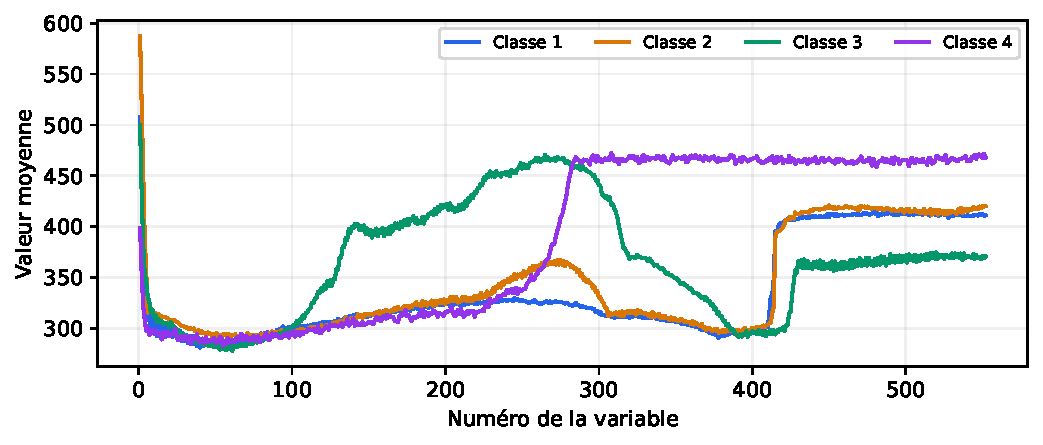
\includegraphics[width=\linewidth,height=5.1cm,keepaspectratio]{aig_profils}
\caption{Profils moyens des quatre classes de référence sur les 552 variables.}
\label{fig:aig-profils}
\end{figure}
Les profils des classes 3 et 4 se distinguent nettement. Ceux des classes 1 et 2
sont proches sur une grande partie des variables, malgré des écarts locaux.
Cette proximité est cohérente avec les désaccords observés entre ces deux classes.


Les trois méthodes sont comparées sans leur fournir les labels ni les effectifs
de référence.

\subsection{Résultats}

Fisher place les débuts des segments 2, 3 et 4 aux observations
\textbf{36, 76 et 121}, soit les intervalles 1--35, 36--75, 76--120 et 121--140 :
ce sont \textbf{exactement les frontières des classes de référence}.

\begin{table}[H]
\centering
\small
\begin{tabular}{@{}lrrrr@{}}
\toprule
\textbf{Méthode} & \textbf{Inertie} & \textbf{ARI / vérité} & \textbf{Silhouette} & \textbf{Changements} \\
\midrule
Fisher  & 10\,457\,795 & \textbf{1,000} & 0,507 & 3 \\
K-means & \textbf{10\,346\,193} & 0,943 & \textbf{0,512} & 9 \\
Ward    & 10\,599\,310 & 0,859 & 0,498 & 7 \\
\bottomrule
\end{tabular}
\caption{Comparaison des trois partitions sur \texttt{aiguillage} ($K=4$).
L'inertie de la partition de référence vaut 10\,457\,795.}
\label{tab:aig}
\end{table}

\begin{itemize}
  \item \textbf{Fisher} reproduit parfaitement la partition de référence (ARI $=1$,
        aucun désaccord).
  \item \textbf{K-means} obtient l'inertie la plus faible mais un ARI de 0,94 :
        3 observations sont mal affectées (22, 67 et 69), toutes entre les classes 1 et 2.
  \item \textbf{Ward} obtient un ARI de 0,86 : 8 désaccords, dont le bloc 19--25
        de la classe 1 rattaché à la classe 2, et l'observation 67.
\end{itemize}
L'ARI entre K-means et Ward vaut 0,87 : les deux méthodes non contraintes
produisent des partitions proches, mais différentes.



\clearpage
\subsection{Visualisation et interprétation}
\begin{figure}[H]
\centering
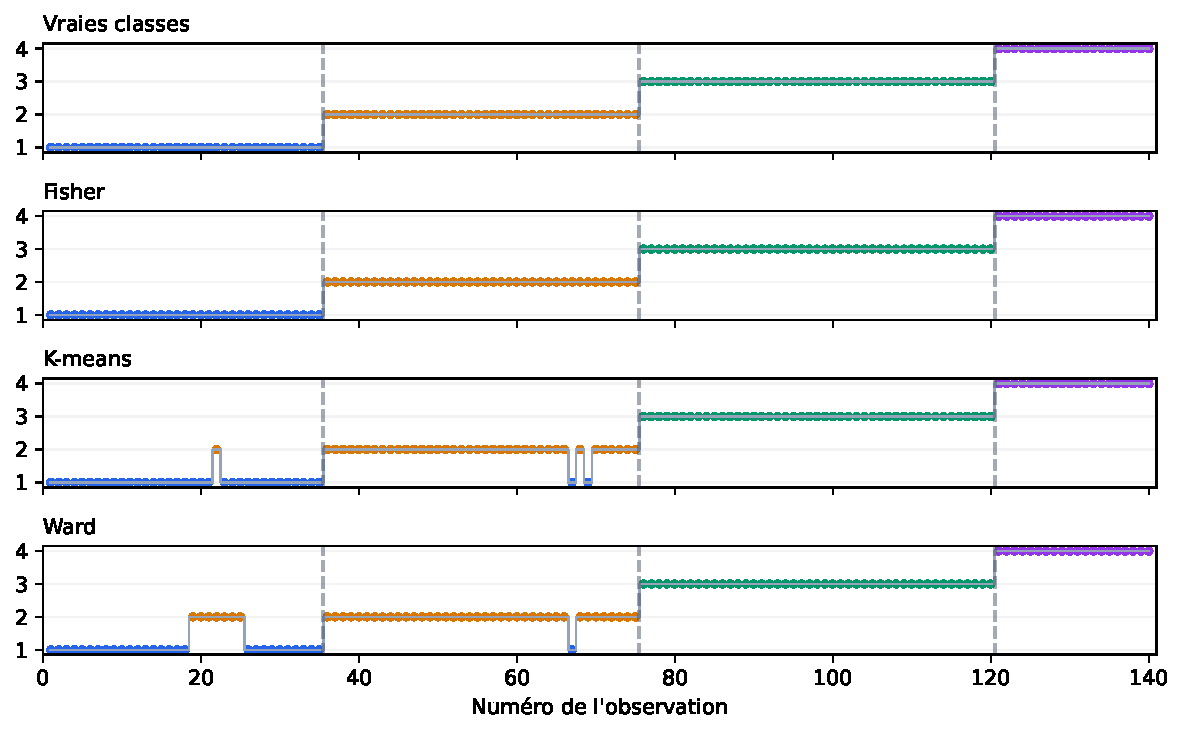
\includegraphics[width=0.95\linewidth,height=6.4cm,keepaspectratio]{aig_sequence}
\caption{Partitions le long de la séquence (classes renumérotées pour
correspondre au mieux aux vraies classes). Pointillés : frontières des vraies classes.}
\label{fig:aig-seq}
\end{figure}

\begin{figure}[H]
\centering
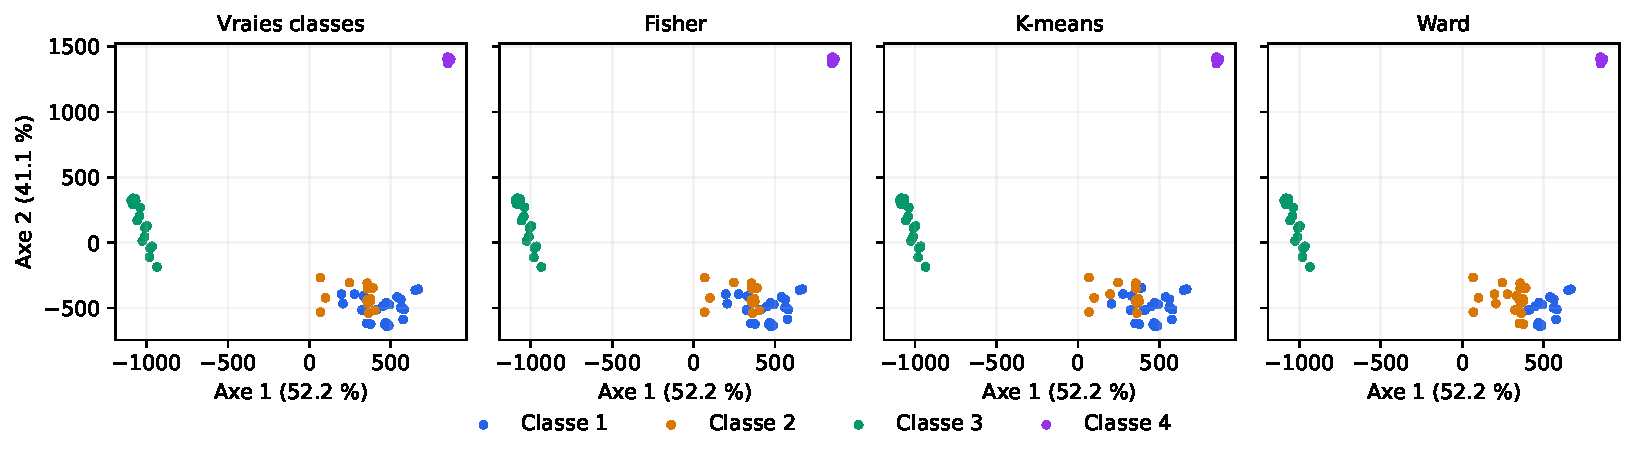
\includegraphics[width=\linewidth,height=5.4cm,keepaspectratio]{aig_acp}
\caption{Projection sur les deux premiers axes de l'ACP (93,3\,\% de la variance).
L'ACP sert uniquement à la visualisation.}
\label{fig:aig-acp}
\end{figure}

La figure~\ref{fig:aig-acp} montre sur ce plan que les classes 3 et 4 sont bien séparées,
alors que les classes 1 et 2 se recouvrent partiellement : c'est dans cette zone
que K-means et Ward se trompent.

\subsection{Compacité et accord avec la vérité}

K-means a une inertie \emph{plus faible} que Fisher tout en étant \emph{moins}
fidèle à la vérité. Ce n'est pas une contradiction : Fisher minimise l'inertie
parmi les seules partitions en segments contigus, alors que K-means cherche dans
un ensemble beaucoup plus grand. Sur ces données, la contrainte d'ordre apporte
une information supplémentaire, la contiguïté des classes, qui permet de lever la
confusion entre les classes 1 et 2.

\subsection{Influence de l'ordre}

Pour vérifier ce rôle de l'ordre, nous avons mélangé aléatoirement les lignes
(cinq fois). L'ARI de Fisher chute alors entre \textbf{0,010 et 0,027}, tandis que
celui de K-means reste à 0,943 sur ces cinq essais : quand les classes ne sont plus contiguës, quatre
segments ne peuvent plus les représenter.

\synthese{\textbf{Bilan \texttt{aiguillage}.} Fisher retrouve exactement les quatre
classes (ruptures 36, 76, 121). K-means et Ward font respectivement 3 et 8 erreurs,
toutes entre les classes 1 et 2. L'avantage de Fisher vient de la contrainte d'ordre,
pertinente ici car les classes se succèdent par blocs.}

% =====================================================================
\clearpage
\section{Discussion}

\subsection{Quand utiliser la contrainte d'ordre ?}

Les deux applications illustrent la même idée sous deux angles :
\begin{itemize}
  \item sur \texttt{aiguillage}, la contrainte d'ordre est \textbf{cohérente avec la
        structure réelle} des données (classes rangées par blocs) et améliore
        l'accord avec la vérité par rapport aux méthodes non contraintes ;
  \item sur \texttt{sequencesimu}, elle permet de \textbf{dater les changements de
        régime} et de distinguer deux périodes aux profils moyens proches, sans supposer
        que leurs distributions soient identiques ;
  \item à l'inverse, l'expérience des lignes mélangées montre que Fisher
        ne retrouve plus les classes de référence lorsque celles-ci ne sont plus
        contiguës, même si elle reste optimale pour son propre critère.
\end{itemize}
Dans nos expériences, les méthodes non contraintes obtiennent souvent de
meilleurs critères internes. Il ne s'agit pas d'une garantie générale : K-means
et Ward ne trouvent pas nécessairement l'optimum global, et n'optimisent pas
la silhouette. Ces critères ne doivent donc pas être le seul élément de comparaison : le nombre de
changements de classe, et surtout la question posée (segmenter une séquence ou
identifier des états), sont déterminants.

\subsection{Limites et pistes d'amélioration}

\begin{itemize}
  \item \textbf{Coût de calcul.} Notre implémentation calcule chaque $D(a,b)$
        directement, soit $O(n^3p)$ opérations pour la matrice $D$. Le calcul reste
        praticable sur les tailles étudiées, mais l'utilisation de sommes cumulées de $x_i$ et
        $\lVert x_i\rVert^2$ ramènerait ce calcul à $O(n^2p)$. La mémoire en
        $O(n^2)$ limite aussi la taille des séquences traitables.
  \item \textbf{Choix de $K$.} La méthode du coude reste une règle visuelle. Elle
        est très nette sur \texttt{sequencesimu}, mais pourrait être ambiguë sur
        des données plus bruitées ; des critères pénalisés avec des hypothèses explicites
        pourraient permettre d'automatiser ce choix.
  \item \textbf{Critère utilisé.} L'inertie euclidienne favorise des groupes compacts autour d'un centre,
        sans imposer formellement une distribution sphérique. Elle est sensible à l'échelle des
        variables : une standardisation peut être nécessaire lorsque les variables
        ne sont pas homogènes.
  \item \textbf{Régimes récurrents.} Fisher attribue une classe différente à chaque
        segment, même lorsque deux segments ont le même comportement. Un
        regroupement \emph{a posteriori} des segments, ou un modèle de Markov caché,
        permettrait d'identifier directement les régimes récurrents.
\end{itemize}

% =====================================================================
\section{Conclusion}
Les 40 tests valident les cas étudiés et confirment, par recherche exhaustive sur
de petites séquences, les coûts optimaux de Fisher. Le coude conduit à quatre
segments sur \texttt{sequencesimu}, dont deux ont des profils moyens proches.
Sur \texttt{aiguillage}, Fisher retrouve les quatre classes connues, tandis que
K-means et Ward présentent trois et huit désaccords.

Fisher répond à un objectif précis : identifier des segments contigus en
exploitant l'ordre des observations. La compacité seule ne garantit pas le
meilleur accord avec une partition de référence. Ces conclusions concernent les
deux fichiers, les valeurs de $K$ retenues et les données brutes ; elles ne
prouvent pas une supériorité générale de Fisher.

\begingroup\small
\begin{thebibliography}{9}
\setlength{\itemsep}{2pt}
\bibitem{fisher} W. D. Fisher (1958). \emph{On Grouping for Maximum Homogeneity}.
Journal of the American Statistical Association, 53(284), 789--798.
\href{https://doi.org/10.1080/01621459.1958.10501479}{doi:10.1080/01621459.1958.10501479}.
\bibitem{sujet} Sujet du projet \emph{Clustering sous contrainte d'ordre},
Master MLSD, 2026--2027, questions 1 à 3.
\bibitem{sklearn} Documentation de scikit-learn : KMeans,
AgglomerativeClustering, adjusted\_rand\_score et silhouette\_score.
\href{https://scikit-learn.org/stable/}{Documentation officielle en ligne}.
\end{thebibliography}
\endgroup
\end{document}
